\section{Methodology}

%------------------------------------------------

\begin{frame}
    \frametitle{Dataset description}
    \vspace{3mm}

	    \begin{columns}
	        % Columna de la izquierda: Texto
	        \begin{column}{0.5\textwidth}
		    \textbf{Data obtained from TCGA Breast Radiogenomics \cite{b3}:}
		       \vspace{2mm}
		    \begin{itemize}
		        \item \textbf{Radiomic Features:}
		        \begin{itemize}
		            \item 36 quantitative features derived from MRI images.
		            \item Shape, texture, etc.
		        \end{itemize}
		        \vspace{2mm}
		        \item \textbf{Multigenic Assay Results:} Genomic scores associated with breast cancer prognosis.
		        \vspace{2mm}
		        \item \textbf{Clinical Data:} Patient demographics, tumor characteristics, and treatment.
		    \end{itemize}
		\end{column}
	        % Columna de la derecha: Imagen
	        \begin{column}{0.4\textwidth}
	            \centering
	            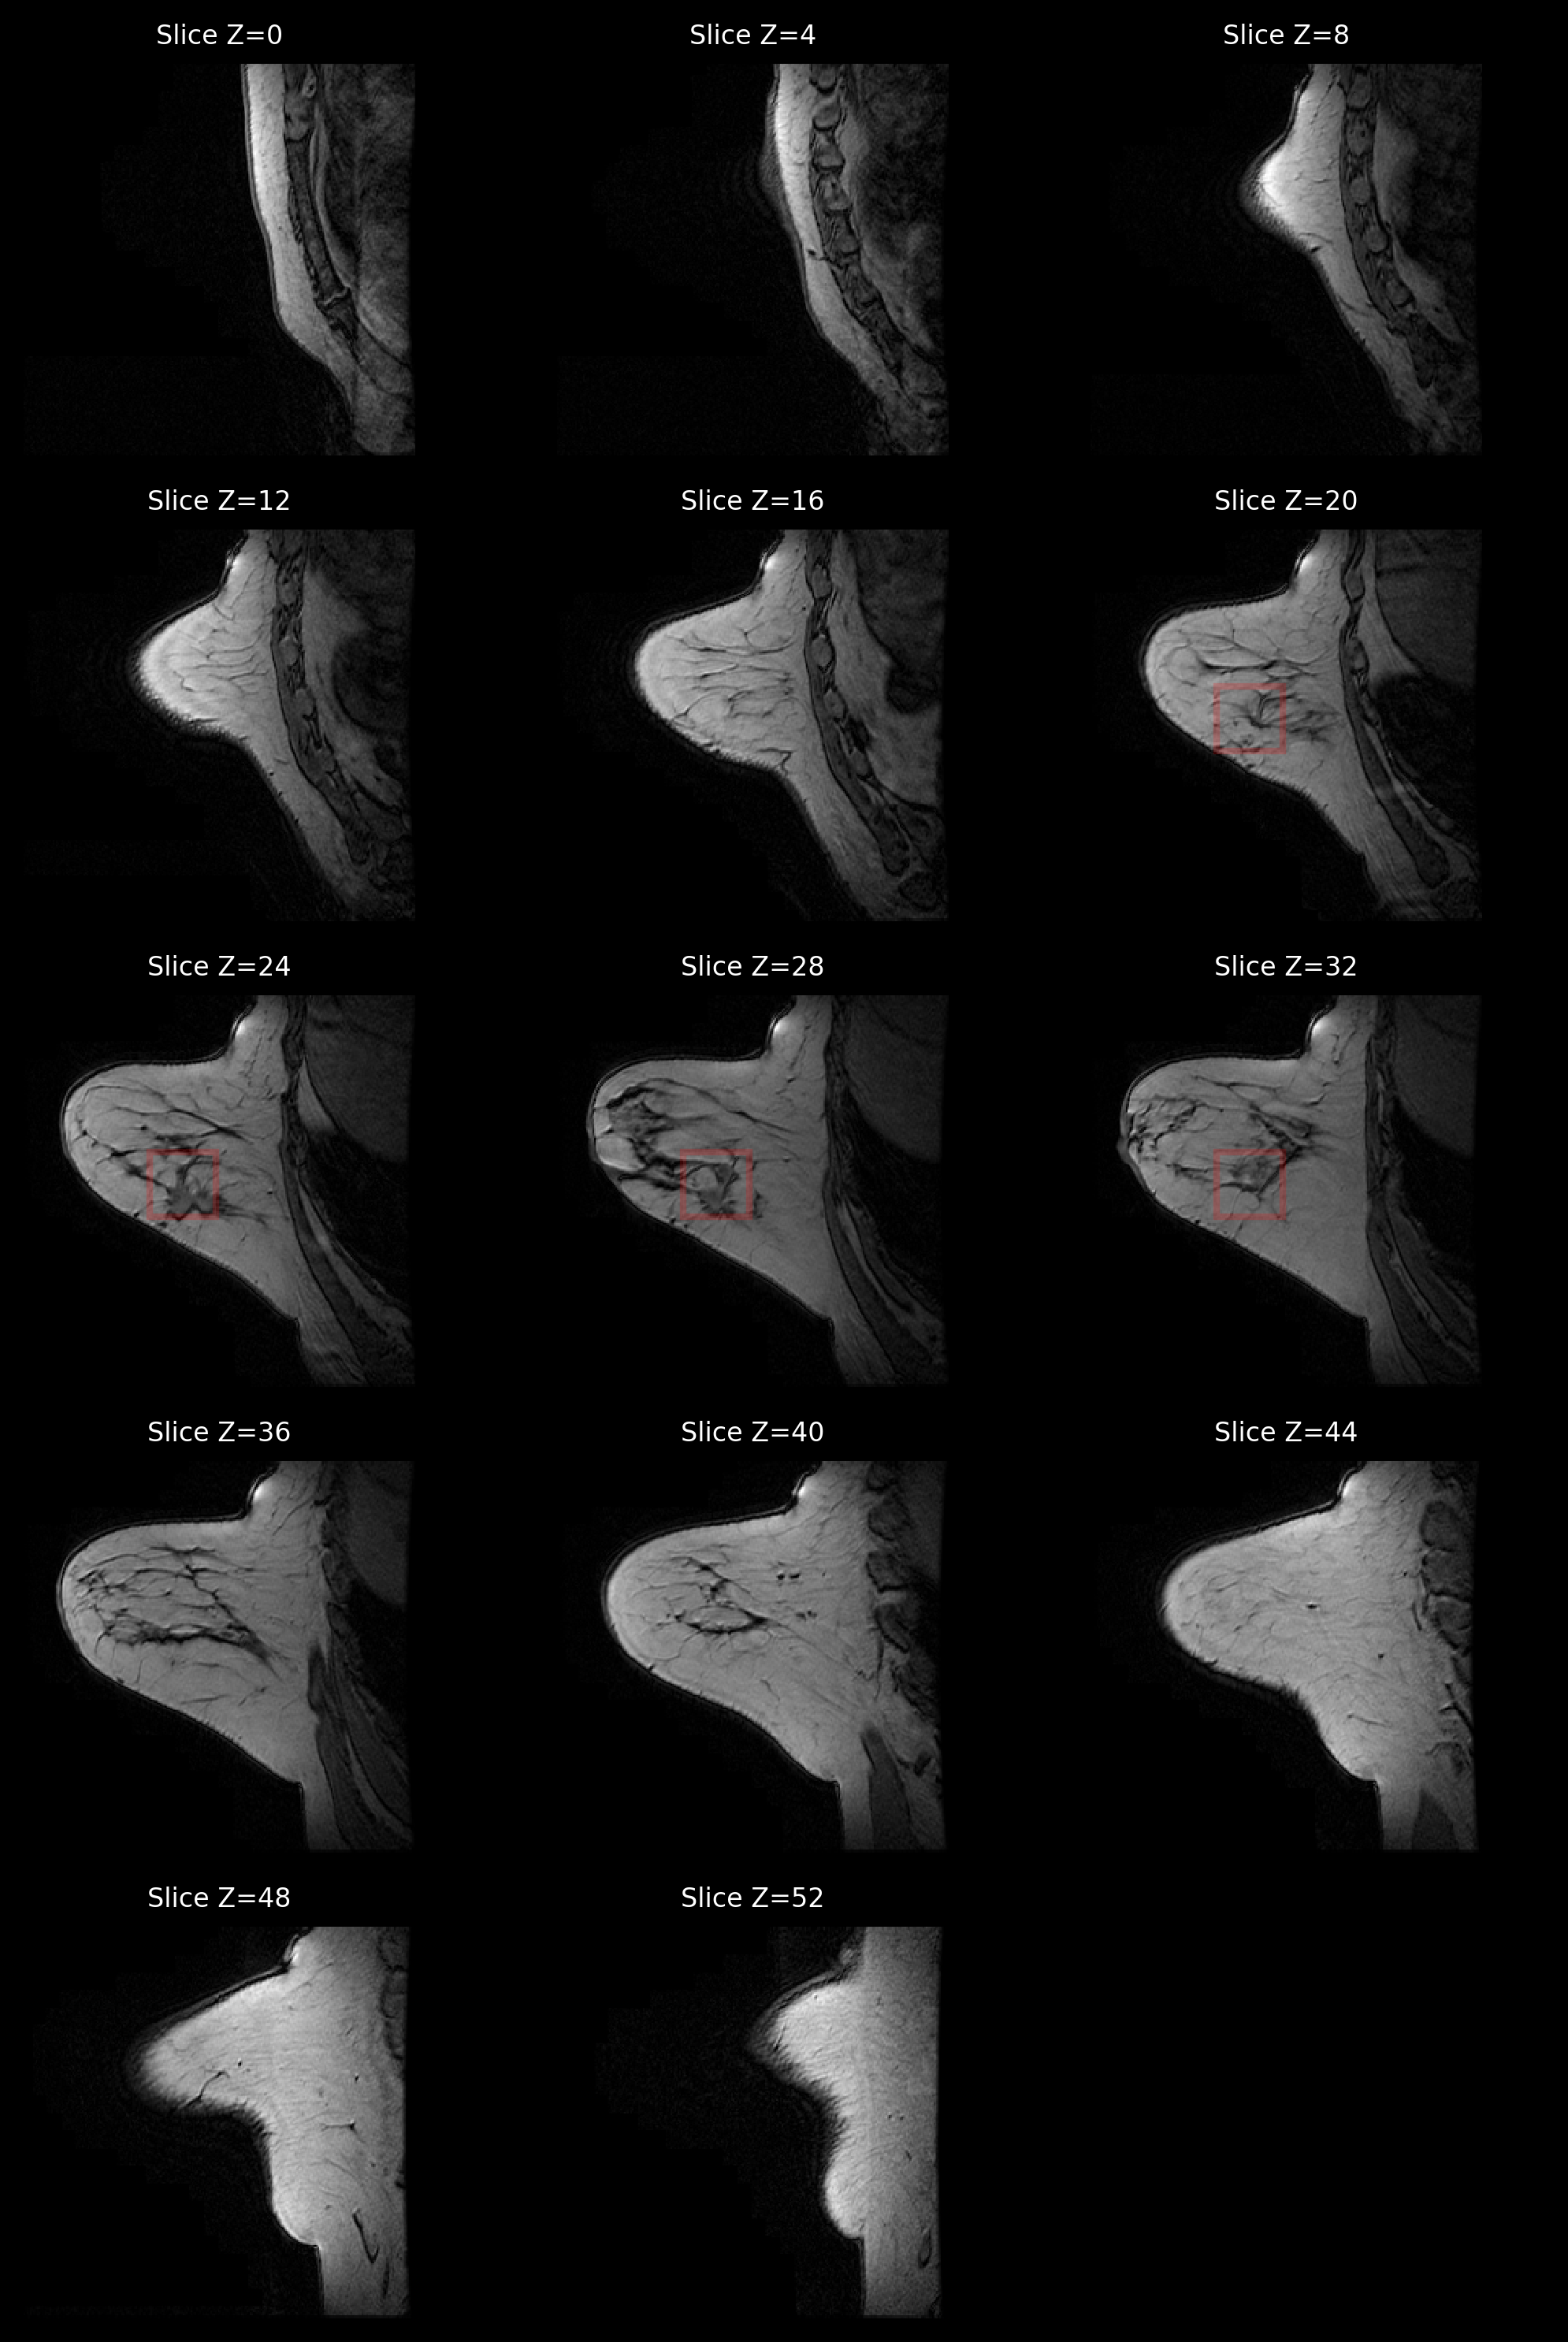
\includegraphics[height=0.85\textheight]{mri_example.png}
	        \end{column}
	    \end{columns}
    \vfill 
\end{frame}

%------------------------------------------------

\begin{frame}
    \frametitle{Data preprocessing I }
    \vspace{3mm}

    \textbf{Preprocessing Steps:}
    \vspace{4mm}
    \begin{itemize}
        \item \textbf{Selection of complete instances:} Only instances with complete information across all datasets are included.
        \vspace{3mm}
        \item \textbf{Removal of the ``Normal" category:} Instances labeled as "Normal" in the \texttt{Pam50.Call} variable are excluded, as they are not relevant for molecular subtype classification.
        \end{itemize}
    \vfill 
\end{frame}

%------------------------------------------------

\begin{frame}
    \frametitle{Data preprocessing II}
    \vspace{3mm}

    \textbf{Result:} After preprocessing, the dataset is reduced from 84 to 76 instances.
    \vspace{5mm}
    \begin{figure}[h]
        \centering
        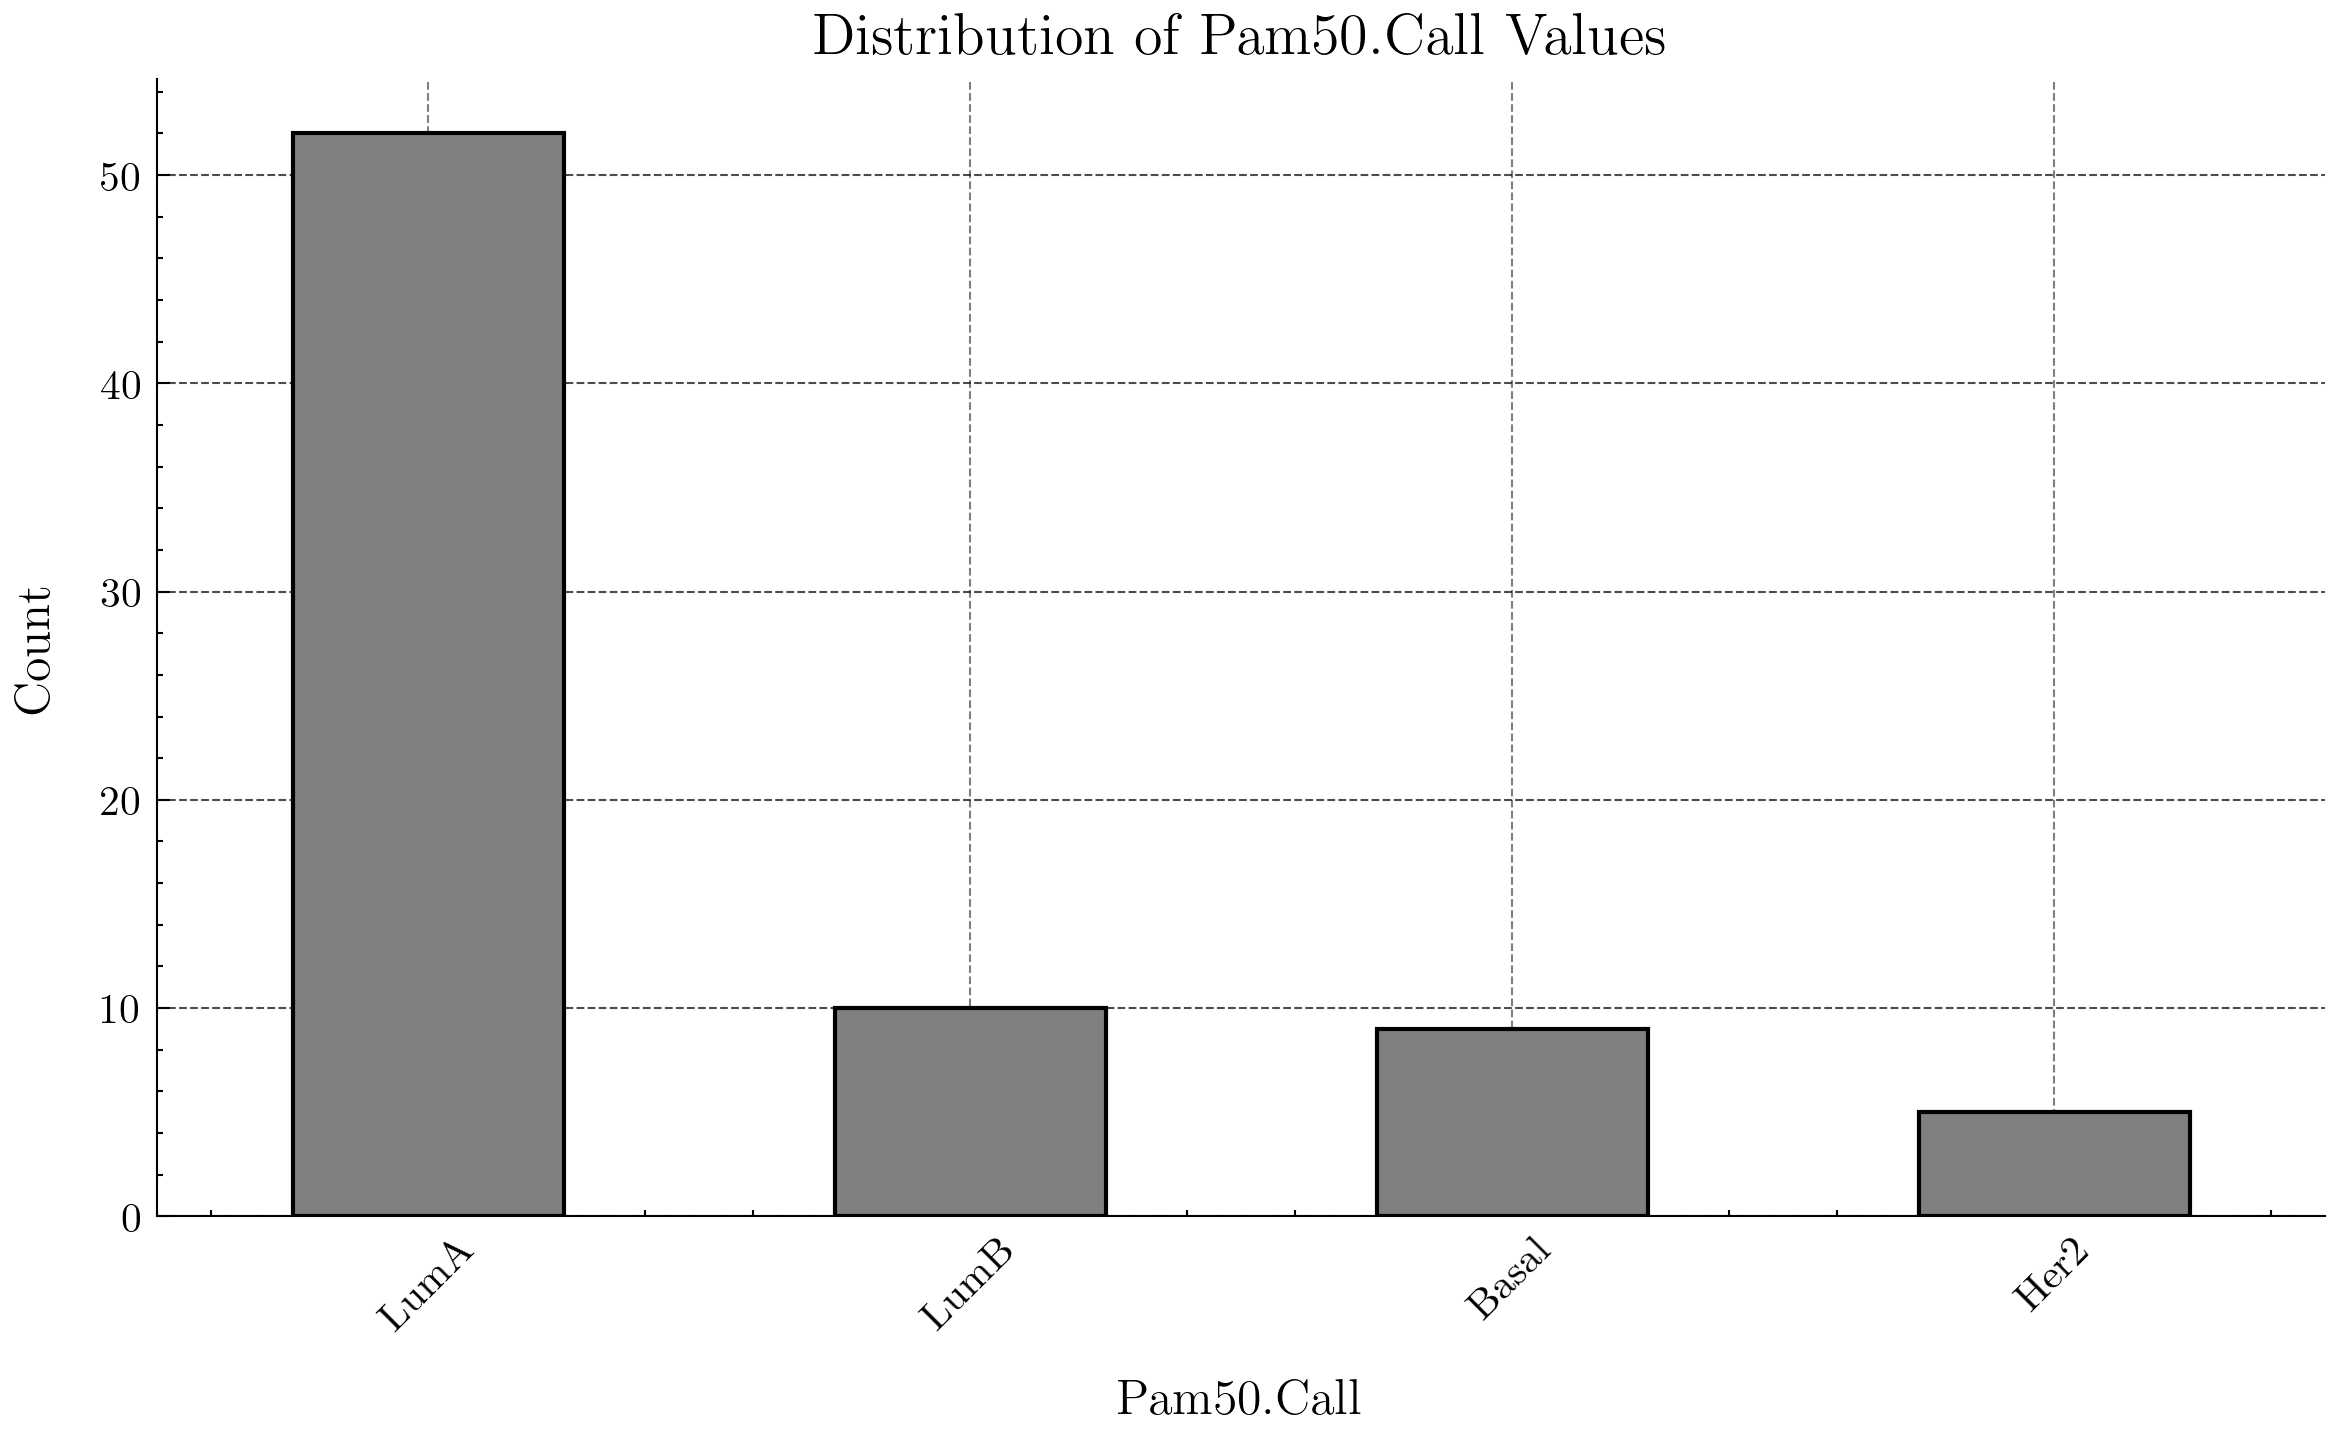
\includegraphics[width=0.75\linewidth]{pam_distr.png}
        \caption{Distribution of the \texttt{Pam50.Call} variable.}
        \label{fig:pam50_distribution}
    \end{figure}

    \vfill 
\end{frame}

%------------------------------------------------

\begin{frame}
    \frametitle{Feature selection}
    \vspace{3mm}

    \textbf{Based on exploratory analysis and medical considerations, the following variables were selected from each dataset:}
    \vspace{3mm}

    \begin{itemize}
        \item \textbf{Clinical Data:}
        \begin{itemize}
            \item \textbf{Age at diagnosis}
            \item \textbf{Cancer stage and tumor size}
            \item \textbf{Number of affected lymph nodes:} Reflects metastatic spread and indicates the severity of the disease \cite{b5}.
            \item \textbf{Hormone receptor status (estrogen and progesterone):} Essential for distinguishing Luminal subtypes \cite{b6}, but also highly correlated with the target variable.
        \end{itemize}

        \vspace{3mm}
        \item \textbf{Multigenic Assay Data:}
        \begin{itemize}
            \item \textbf{GHI RS Score:} Continuous score from the Oncotype DX assay measuring recurrence risk \cite{b7}. 
            \item \textbf{Correlation with good outcome signature:} Indicates how strongly the sample correlates with a favorable prognosis gene profile from the MammaPrint assay \cite{b8}.
            \item \textbf{Proliferation-related gene expression:} Represents the average expression of genes linked to cell proliferation.
        \end{itemize}
    \end{itemize}

    \vfill 
\end{frame}